% -*- coding: UTF-8 -*-
% vim: autoindent expandtab tabstop=4 sw=4 sts=4 filetype=tex
% vim: spelllang=de spell
% chktex-file 27 - disable warning about missing include files

\section{Klassendiagramme}
\label{sec:class-diagrams}

Klassendiagramme sind Teil des Design-Modelles und illustrieren Klassen,
Interfaces und deren Beziehungen~\cite[S. 249 bis 251]{larman_applying_2004}.
Sie sind also eine grafische Darstellung der statischen Sicht einer
Software~\cite[S. 217]{rumbaugh_unified_2004}. Ein Klassendiagramm beinhaltet
diverse konkrete Elemente, welche auf das Verhalten der Software bezogen sind,
wie zum Beispiel Methoden. Deren Dynamik wird allerdings in anderen Diagrammen,
wie dem Statechart-Diagramm oder dem Kommunikations-Diagramm
festgehalten~\cite[S. 217]{rumbaugh_unified_2004}.

Die Notation ist dieselbe oder zumindest sehr ähnlich wie bei dem
Domänenmodell. Letzteres zeigt aber mehr eine konzeptuelle Sicht.
Domänenmodelle können als Klassendiagramme aus einer konzeptuellen Sicht
bezeichnet werden~\cite[S. 249]{larman_applying_2004}. Klassendiagramme selbst
repräsentieren also mehr eine Software-Sicht und daher einen Teil der
Implementation.

Wie bereits in den vorherigen Modell, fehlen auch hier einige essentielle
Konzepte beziehungsweise Objekte bewusst.  Diese werden während den Iterationen
der darauffolgenden Projektarbeit erarbeitet. Ein Teil ist im Player
angedeutet, ein anderer Teil im Editor. Würde man das gesamte Klassendiagramm
abbilden wollen, würde dies schnell unübersichtlich. Ein weiterer Teil findet
sich im Klassendiagramm des Prototypen (\ref{chap:prototype}). Ein
detaillierteres Bild der Klassen wird bei den einzelnen Iterationen bzw.\
Phasen (Elaboration, Construction und Transition) im Rahmen der darauffolgenden
Projektarbeit noch im Detail erarbeitet. Gegebenenfalls ist es dort dann jedoch
sinnvoller nur Ausschnitte pro Paket zu zeigen und die Interaktion zwischen den
Schichten mittels Interfaces darzustellen.

Abbildung~\ref{fig:class-diagram:player} zeigt das Klassendiagramm des
Players, Abbildung~\ref{fig:class-diagram:editor} dies des Editors.

Die verschiedenen Pakete respektive Layer wurden farblich unterschieden. Die
farblichen Konventionen sind die folgenden:

\begin{itemize}
    \item[]\img[30pt]{img/ui_node.png}
        \textit{UI}:\@ Alle Elemente der grafischen Benutzeroberfläche.
    \item[]\img[30pt]{img/app_node.png}
        \textit{Application}:\@ Controller / Workflow-Objekte.
    \item[]\img[30pt]{img/domain_node.png}
        \textit{Domain}:\@ Modelle / Applikationslogik.
    \item[]\img[30pt]{img/tech_node.png}
        \textit{Technical services}:\@ Technische Infrastruktur wie Grafik, Erzeugung von
        Fenstern etc.
    \item[]\img[30pt]{img/foundation_node.png}
        \textit{Foundation}:\@ Grundlegende Elemente, low-level technical services wie
        Timer, Array oder andere Datenklassen.
\end{itemize}

\begin{figure}[H]
    \centering
    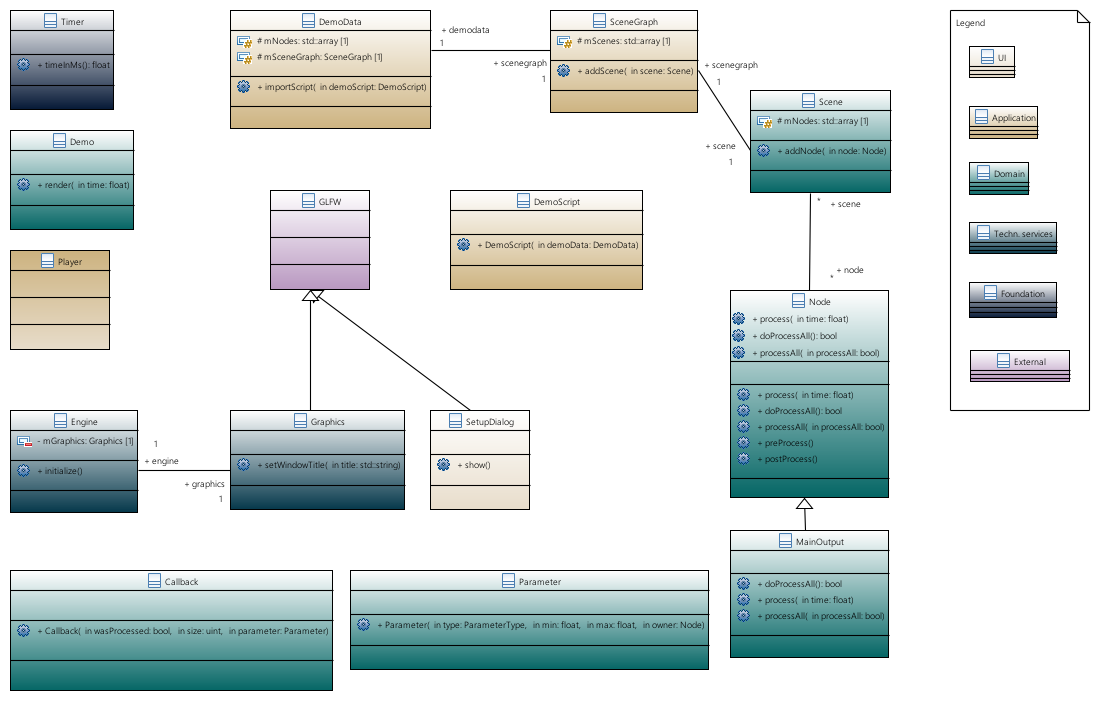
\includegraphics[width=0.8\textwidth]{img/player_class_diagram.png}
    \caption{Klassendiagramm der
        Player-Applikation\protect\footnotemark}\label{fig:class-diagram:player}
\end{figure}
\footnotetext{Eigene Darstellung mittels Papyrus.}

\begin{figure}[H]
    \centering
    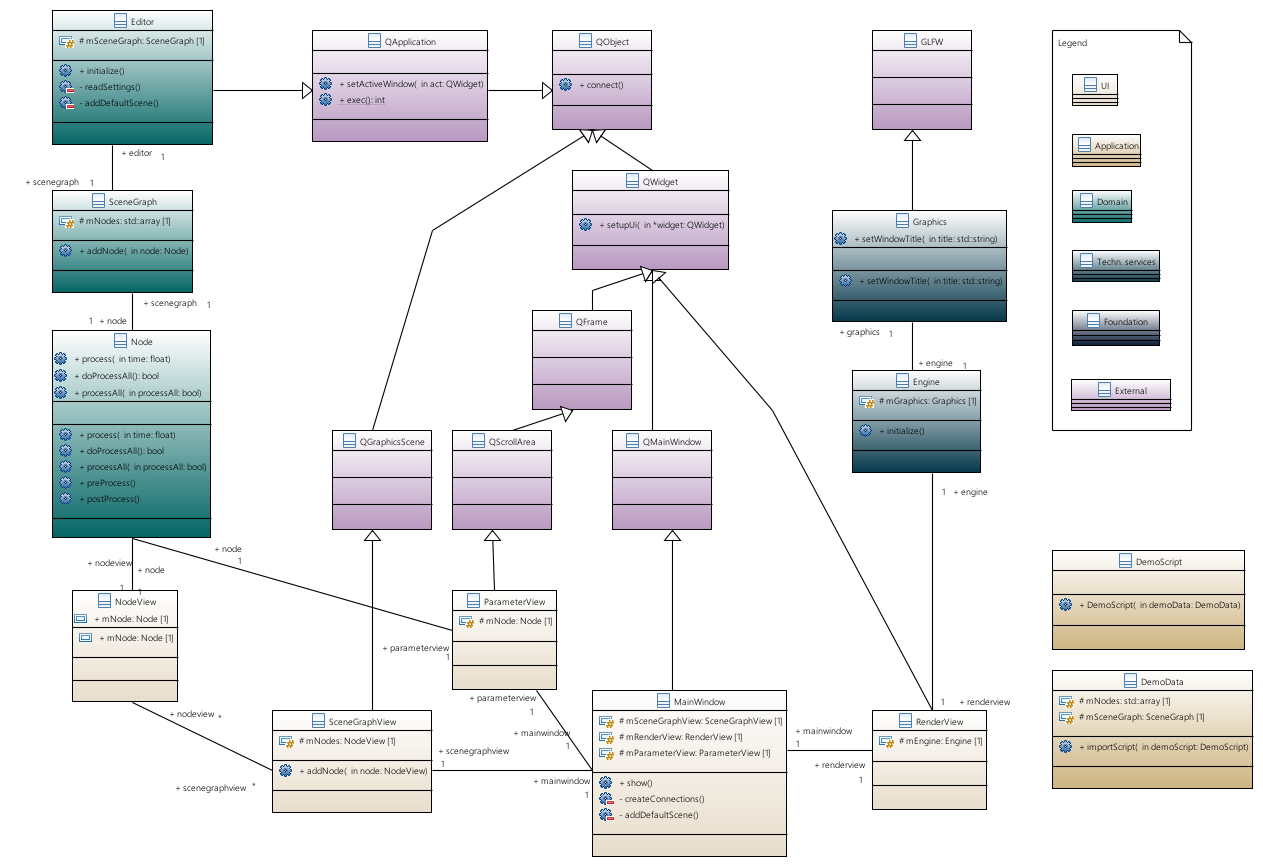
\includegraphics[width=1.0\textwidth]{img/editor_class_diagram.png}
    \caption{Klassendiagramm der
        Editor-Applikation\protect\footnotemark}\label{fig:class-diagram:editor}
\end{figure}
\footnotetext{Eigene Darstellung mittels Papyrus.}
